%
% Forschungsstand:
%
% - Welche wissenschaftlichen Erkenntnisse liegen zu dem Thema bereits vor?
% - Grundsätzlich gibt es zwei Möglichkeiten, einen Forschungsstand zu schreiben: Entweder ordnen Sie Ihren Literaturüberblick nach Themenkomplexen oder Sie geben einen rein chronologischen Überblick über die wichtigsten Publikationen.
% - Auf keinen Fall sollten Sie den Forschungsstand zu voll packen. Es geht nicht darum, dem Leser zu zeigen, was Sie alles studiert haben (wie fleißig Sie waren), sondern um einen kompakten Überblick über die wichtigste Literatur.
% - Wichtig: Listen Sie die Literatur nicht nur auf, sondern erklären Sie, welchen Beitrag die jeweilige Publikation zum Erkenntnisgewinn geleistet hat. Also, zum Beispiel: Was hat der Autor als Erster erkannt oder hinterfragt? Es muss ja einen Grund geben, weshalb Sie die betreffende Publikation unter die Meilensteine reihen – und den sollten Sie dem Leser deutlich machen.
%
% Ferrein:
% - 4-5 Seiten in der Bachelorarbeit (deutlich umfangreicher als im Exposé)
% - Was unterscheidet meinen Ansatz von den anderen verhandenen Ansätzen?
%

\begin{comment}
------------------------------------------------------------------------------------------
- Informationen aus dem Expose
	- Einen guten Überblick über die Eigenschaften der Drahtlosen-Protokolle (engl. Wireless Protocols) Bluetooth, UWB, ZigBee und WiFi liefert die Arbeit \cite{lee2007comparative} von \citeauthor{lee2007comparative}.
	- In \cite{smith1987closed} wird das grundlegende Prinzip erklärt um aus mehreren bekannten Sensoren die Position eines beweglichen Empfängers zu berechnen.
	- Der theoretische Hintergrund des SLAM--Verfahrens wird in \cite{dissanayake2001solution} vorgestellt. Zusätzlich wird bewiesen das die Unsicherheit bei der Kartenerstellung und Lokalisierung eine untere Schranke erreicht.
	- \citeauthor{kantor2002preliminary} stellen in Ihrer Arbeit \cite{kantor2002preliminary} ein Lokalisierungsverfahren vor, welches die Roboterposition anhand von Entfernungsmessungen zu vorher bekannten Landmarken bestimmen kann. Im letzten Abschnitt wird SLAM--Verfahren vorgestellt, welches über einen Kalman--Filter die Unsicherheit der Landmarkenposition modellieren kann.
	- Die Autoren \citeauthor{blanco2008pure} gehen in ihren Arbeiten \cite{blanco2008pure, blanco2008efficient} einen Schritt weiter und bestimmen die unbekannte Roboterposition sowie die unbekannten Landmarkenpositionen. Hierzu nutzen Sie im ersten Schritt einen Partikelfilter (engl. Particle Filter) bis die Schätzung eine ausreichende Genauigkeit erreicht hat um dann im zweiten Schritt über einen Kalman--Filter ein Positionsverfolgung (engl. Position Tracking) durchzuführen.
	- Die Arbeit \cite{ledergerber2015robot} von \citeauthor{ledergerber2015robot} gehen auf die Roboterlokalisierung unter Verwendung einer One-Way Ultra-Wideband Kommunikation ein. Dieses hat den Vorteil, das mit sehr wenigen Landmarken eine große Anzahl von Roboter lokalisiert werden kann.
	
	- The Cartesian EKF described above operates in the Cartesian space, we formulate our problem in polar coordinates.
	
	- The use of this parameterization derives motivation from the polar coordinate system, where annuli, crescents and other ringlike shapes can be easily modeled. This parameterization is called Relative Over Parameterized (ROP) because it over parameterizes the state relative to an origin.

	- EKF -> Polar EKF -> Multi-Hypothesis Filter
	
	- Partikel Filter
\end{comment}


\begin{comment}
------------------------------------------------------------------------------------------
\end{comment}
\chapter{Stand der Forschung und Technik [rework]}

In diesem Kapitel wird ein chronologischer Überblick über die wichtigsten Publikationen zum Thema \Gls{roslam} geliefert. Jeder Autor verwendet eine etwas andere Terminologie, auch wenn es sich im Kern um die gleiche Sache handelt. Daher werden in diesem Kapitel die Begriffe Anker, Tag und Beacon synonym verwendet.


\begin{comment}
------------------------------------------------------------------------------------------
- \cite{kantor2002preliminary}
- Preliminary results in range-only localization and mapping (189)
- Section 2
	- Statische Lokalisierung
		- Vorherige Sensorinformationen und Positionsschätzung werden nicht genutzt.
		- Annahme: Position der Beacons ist bekannt und fix.
	- Markovian probability grids
	- Mit fehlerfreien Messungen ist die Positionsbestimmung trivial
	- Entfernungsmessung mit einem erwarteten Fehler von 6 feet, also 1,82 meter. (1Fuß==30cm)
	- 1. Characterizing Range Measurements
		- Erstellen einer Verteilungsfunktion für die Entfernungsmessung
		- experimentel bestimmt
		- Diskrete Messungen in einem Set {0,6,12,...,50}
	- 2. Creating Probability Grids
		- Für jede Zelle des Grid wird die Wahrscheinlichkeit mittels der PDF berechnet.
	- 3. Combine Probability Grids
		- Multiply in a pointwise manner
		- scale the result so that the sum over the squares is one.
		- Aus den kombinierten Ergebnisgrid kann die schätzte Position mittels der gewichteten Durchschnitt der Gridzellen berechnet werden.
		- Covariance Matrix lässt sich auch bestimmen
	- Durchschnittlich geschätzer Fehler lag ab 1,62 feet bei einem geschätzen Entfernungsmess Fehler von 5.82 bis 7.18 feet.
- Section 3
	- Beacon positionen sind bekannt
	- Vorherige Positionsschätzung und Odometry daten werden verwendet.
	- Positionsverfolgung mittels Kalman und Monte Carlo
	- Kalman
		- Initiale Positionsschätzung wie in Section 2, jedoch mit drei Beacons.
		- Approximieren eines ringförmigen Gauß-Verteilung um die geschätzte Position.
		- Füttern eines entsprechenden EKF mit den Parametern
	- Monte Carlo
		- Verwendet die pdf aus Section 2 um die Partikels zu gewichten.
	- Durchschnittliche Geschätzter Fehler
		- EKT: 0,73 feet
		- MC: 0,93 feet
- Section 4
	- Lokalisieren in einer Umgebung mit unsicheren beacon positionen
		- Approximately known, good but not perfect
		- crude measurement or estimate location on blueprint
	- SLAM mit EKF
		- State ist die Robot-- und Beacon--Position
		- Error: init 5.13 feet, end 0.77 feet
\end{comment}
\section{Preliminary results in range-only localization and mapping}

In \citetitle{kantor2002preliminary}\cite{kantor2002preliminary} verwendet der Author \Glspl{beacon} die eine Entfernungsschätzung mit einem mittleren Fehler von \SI{1.82}{\metre} (6 Fuß) liefern. Um das Problem der Datenzuordnung zu trivialisieren, liefert jeder \Gls{beacon} zusätzlich zur Messung eine eindeutigen Identifikationsnummer mit. Nur mit diesen Daten werden die Probleme der Roboter Lokalisierung, Positionsverfolgung und \Gls{slam} behandelt. Das algorithmische Fundament wird dabei durch den \Gls{ekf} und \Gls{mc} Partikelfilter gebildet.

Im ersten Abschnitt wird die statische Lokalisierung thematisiert, die für eine Positionsschätzung auf vorherige Sensorinformationen und Positionsschätzungen verzichtet. Bei einer fehlerfreien Entfernungsmessungen ist die Positionsbestimmung ein mathematisch triviales Problem. Da die Messungenauigkeit mit \SI{1.82}{\metre} jedoch sehr hoch ist, werden Methoden der Wahrscheinlichkeitstheorie verwendet. Im ersten Schritt wird die Verteilungsfunktion experimentell für einige diskreten Abstände bestimmt. Unter zuhilfenahme der erstellten Verteilungsfunktion wird für jeden \Gls{beacon} und für jede Zelle des \Gls{propgrid} die Wahrscheinlichkeit berechnet, siehe \figurename~\ref{fig:kantor2002preliminary_figure1b} links. Im letzten Schritt werden die einzelnen \Gls{propgrid} miteinandern multipliziert und im Abschluss skaliert damit die Summe über alle Zellen gleich eins ist, siehe \figurename~\ref{fig:kantor2002preliminary_figure1c} rechts. Aus dem gewichteten Durchschnitt der Zellen lässt sich die Position schätzen, siehe \figurename~\ref{fig:kantor2002preliminary_figure1c}. Der durchschnittliche Schätzungsfehler beträgt \SI{0.49}{\metre} bei einem erwarteten Fehler von \SIrange{1,77}{2,18}{\metre} bei der Entfernungsmessung.

\begin{figure}[htbp]
  \begin{minipage}[t]{0.45\linewidth}
    \centering
    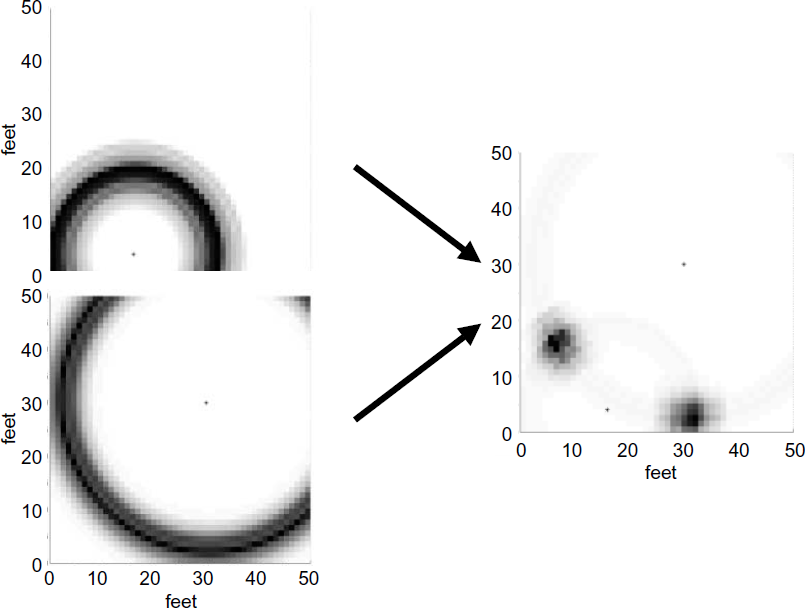
\includegraphics[width=\linewidth]{kantor2002preliminary_figure1b}
    \caption{Links: \Gls{propgrid} pro \Gls{beacon}. Rechts: Kombination zweier \Glspl{propgrid}.}
    \label{fig:kantor2002preliminary_figure1b}
  \end{minipage}
  \hfill
  \begin{minipage}[t]{0.45\linewidth}
    \centering
    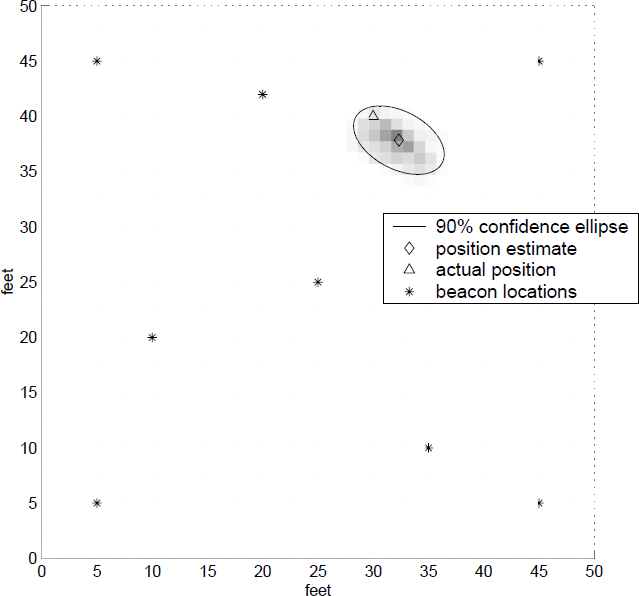
\includegraphics[width=\linewidth]{kantor2002preliminary_figure1c}
    \caption{Kombiniertes \Gls{propgrid} aller \Glspl{beacon}.}
    \label{fig:kantor2002preliminary_figure1c}
  \end{minipage}
	\source{\cite{kantor2002preliminary}}
\end{figure}

Im nächsten Abschnitt wird die Positionsverfolgung mittels eines \Gls{ekf} bzw. \Gls{mc} Partikelfilter behandelt. Hier für werden die Odometriedaten und die vorhergie Positionsschätzung verwendet. Für eine initiale Positionsschätzung wird das Verfahren aus dem vorherigen Abschnitt verwendet. Aus der Entfernungsschätzung eines \Glspl{beacon} ergibt sich eine ringförmige Verteilungsfunktion, die mit einer unimodalen Verteilung nicht modelliert werden kann. Als Annäherung wird eine Normalverteilung verwendet, die in tangentialer Richtung gestreckt und in radialer Richtung gestaucht ist. Als Mittelwert wird die vorherige Positionsschätzung verwendet, siehe \figurename~\ref{fig:kantor2002preliminary_figure2}. Um die Partikel im \Gls{mc} Partikelfilter zu gewichten ist die ringförmige Verteilung vollkommen ausreichend. Der durchschnittliche Schätzungsfehler beträgt beim \Gls{ekf} \SI{0.22}{\metre} und \SI{0.28}{\metre} beim \Gls{mc} Partikelfilter.

\begin{figure}[htbp]
	\centering
	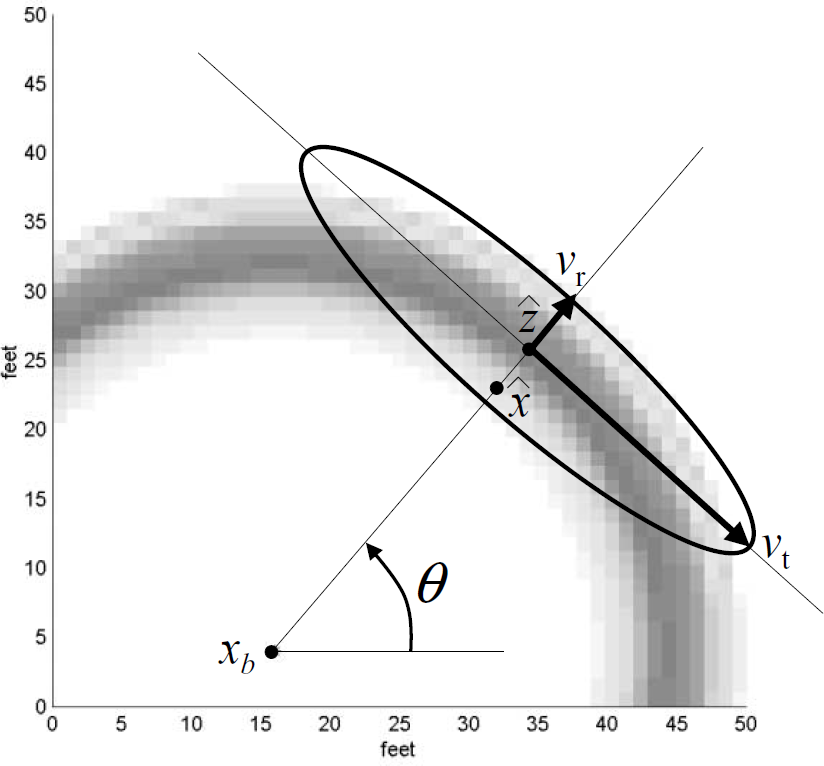
\includegraphics[width=0.5\linewidth]{kantor2002preliminary_figure2}
	\caption{Annäherung einer ringförmigen Verteilung an eine Normalverteilung.}
	\label{fig:kantor2002preliminary_figure2}
	\source{\cite{kantor2002preliminary}}
\end{figure}

Der letzte Abschnitt wird ein \Gls{slam}--Verfahren mittels einem \Gls{ekf} behandelt. Die initiale Roboter-- und \Gls{beacon}--Position muss nicht genau jedoch ungefähr bekannt sein. Der Zustandsvektor des \Gls{ekf} beinhaltet die Roboter-- und alle \Gls{beacon}--Positionen. Der durchschnittliche Fehler in der initalen Schätzung beträgt \SI{1.56}{\metre} und verbessert sich zum Schluss hin auf \SI{0.23}{\metre}.


\begin{comment}
------------------------------------------------------------------------------------------
- \cite{kurth2003experimental}
	- Experimental results in range-only localization with radio (82)
\end{comment}
%\section{Experimental results in range-only localization with radio [todo]}


\begin{comment}
------------------------------------------------------------------------------------------
- \cite{olson2004robust}
	- Robust range-only beacon localization (264)
	- Wie funktioniert die Exploration Strategy?
		- Die Ungünstigeste strategy ist das geradeausfahren mit einem beacon links und rechts.
		- Das Gradientenfeld der abstanddifferenz zwischen den beiden beacons führt einen auf den optimalen weg um die Abstandsdifferenz zu maximieren. (Aktive Exploration)
\end{comment}
\section{Robust range-only beacon localization}

In \citetitle{olson2004robust}\cite{olson2004robust} werden autonome Unterwasserfahrzeuge (engl. \gls{auv}) verwendet um den Ozeanen der Welt die letzten Geheimnisse zu entlocken. Hierfür ist eine genaue Lokalisierung der \gls{auv} notwendig. Dies wird über die Messung der Signallaufzeit zwischen dem \gls{auv} und mehreren stationären akustischen Transponder--\Gls{beacon} erreicht. Vor der eigentlichen Messung müssen jedoch die \Glspl{beacon} im Messbereich verteilt werden, deren Position genau bestimmt werden und zusätzlich dafür gesorgt werden, dass die \Glspl{beacon} ihre Position nicht ändern. Dadurch handelt es sich um ein sehr kostspieliges Prozedere und soll in dem vorgestellt Verfahren dahingehend optimierte werden, dass die \Gls{beacon}--Position vorher nicht bekannt sein muss. Dadurch ist eine autonome Verteilung der \Glspl{beacon} möglich und zusätzlich kann auch detektiert werden ob ein \Gls{beacon} seine Position verändert hat.

% TODO: Spectral Graph Partitioning Übersetzung? 
Bevor jedoch die Laufzeitmessungen verwendet werden können, müssen diese um \Gls{outlier} (dt. Ausreißer) bereinigt werden. Diese entstehen z.B. durch unterschiedliche Ausbreitungsgeschwindigkeiten der Schallwellen im Wasser, durch Reflektionen am Meeresgrund (engl. \Gls{multipath}) oder durch Interferenzen der Nutzlast (engl. \Gls{payload}) mit den Sensoren. Die Bereinigung der Messdaten erfolgt hierbei über das \textit{Spectral Graph Partitioning} Verfahren. Hierbei wird jede Messung als Kreis dargestellt. Überschneiden sich zwei Kreise gelten diese beiden Messungen als konsistent. Jede der Messungen wird in einem Graphen zu einem Vertex und jede konsistente Messung zu einer Kante. Bei dem fertigen Graphen ist nun zu beobachten, dass \Gls{outlier} weniger stark untereinander verbunden sind als \Gls{inlier}. Diese durchschnittliche Konnektivität der \Gls{inlier} wir als Metrik für den Partitionierungsalogorithmus verwendet um die Messdaten zu filtern.

Nach dem die Messwerte pro \Gls{beacon} gefiltert worden sind, werden zwei Messwerte von zwei verschiedenen \Glspl{beacon} wieder mit einandern überschnitten. Hieraus entstehen zwei mögliche Positionen des \gls{auv}. In einem Grid erhöhen diese beiden Positionen dann den Ihnen zugeordneten Zähler. Dieser Vorgang wird für weiter Messwerte wiederholt. Durch das daraus resultierende Voting--System entstehen zwei Gipfel (engl. Peak) die die mögliche Position des \gls{auv} approximieren. Ist der Höhenunterschied zwischen den Gipfeln ausreichend groß, wird die \gls{auv}--Position mit dem höchsten Gipfel an einen EKF--SLAM übergeben.


\begin{comment}
------------------------------------------------------------------------------------------
-\cite{smith2004tracking}
	- Tracking moving devices with the cricket location system (547)
\end{comment}
%\section{Tracking moving devices with the cricket location system [todo]}


\begin{comment}
------------------------------------------------------------------------------------------
\end{comment}
\section{A pure probabilistic approach to range-only SLAM}\label{sec:blanco2008pure}

Alle zuvor vorgestellten Verfahren hatten den Nachteil, dass sie probabilistische und nicht probabilistische Verfahren gemeinsam verwendeten um eine initiale Schätzung der \textit{Beacon}--Positionen zu erlangen. In dieser Initialisierungsphase waren alle Positionsinformationen für die Positionsschätzung des Roboters verloren. In der Arbeit \citetitle{blanco2008pure} \cite{blanco2008pure} wird zu jedem Zeitpunkt die beste \textit{Beacon}--Schätzung genutzt um die Roboterposition zu verbessern. Um das zu bewerkstelligen, wird ein rein probabilistisches Verfahren genutzt.

Verwendung findet hierbei der \Gls{rbpf}, der die Berechnung des Roboterpfades von der Karte mit den Landmarken entkoppelt \cite{murphy2001rao, montemerlo2002fastslam}. Jeder Partikel des \Gls{rbpf} beschreibt dabei pro \textit{Beacon} die Verteilung die am besten zu seiner Positionsschätzung passt. Die Verteilung wird dabei zuerst von einem Hilfspartikelfilter (engl. Auxiliary Particle Filter) modelliert. Seine Partikel besitzen dabei eine ringförmige Verteilung mit dem Abstand des \textit{Beacon}, siehe \figurename~\ref{fig:blanco2008pure_fig3e}. Partikel mit einer geringen Wahrscheinlichkeit werden über eine Gewichtung aussortiert, siehe \figurename~\ref{fig:blanco2008pure_fig3f}. Sobald der Hilfspartikelfilter gegen eine bestimmte \textit{Beacon}--Position konvergiert ist, wird dieser in einen Normalverteilung umgewandelt und über einen \Gls{ekf} modelliert, siehe \figurename~\ref{fig:blanco2008pure_fig3g}.

\begin{figure}
	\begin{subfigure}[t]{0.3\linewidth}
		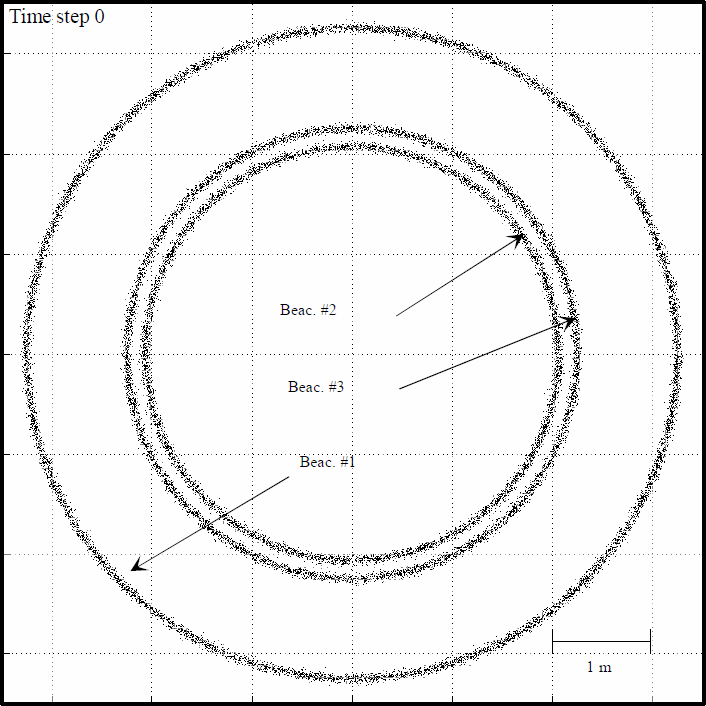
\includegraphics[width=\linewidth]{blanco2008pure_fig3e}
		\caption{}
		\label{fig:blanco2008pure_fig3e}
	\end{subfigure}
	\hfill
	\begin{subfigure}[t]{0.3\linewidth}
		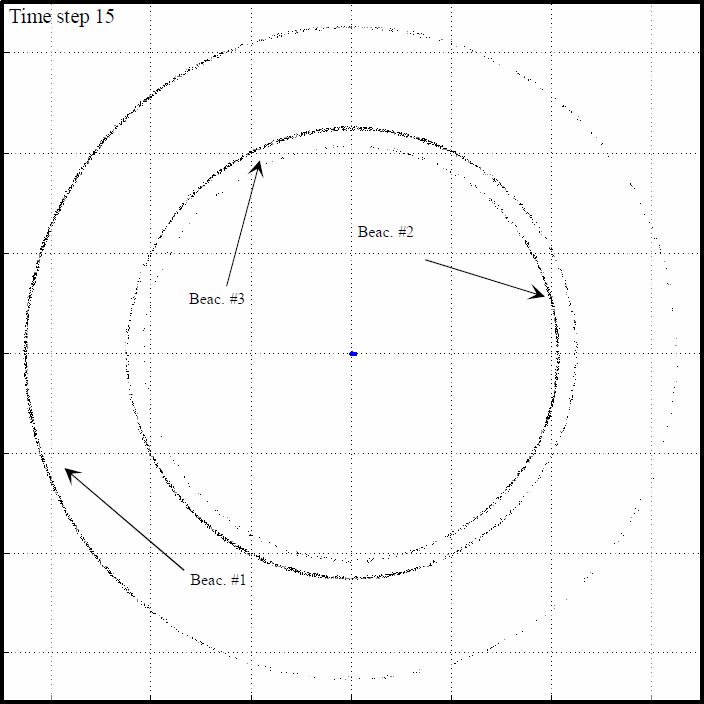
\includegraphics[width=\linewidth]{blanco2008pure_fig3f}
		\caption{}
		\label{fig:blanco2008pure_fig3f}
	\end{subfigure}
	\hfill
	\begin{subfigure}[t]{0.3\linewidth}
		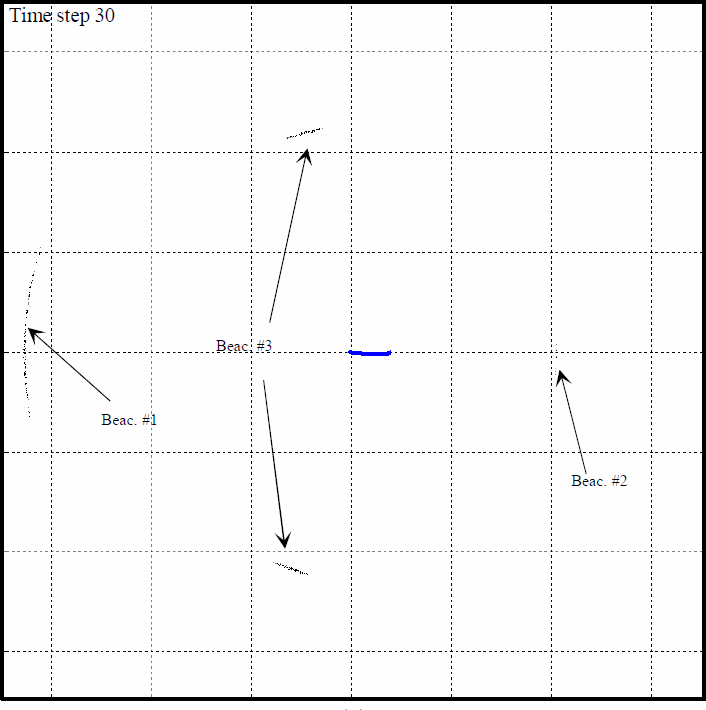
\includegraphics[width=\linewidth]{blanco2008pure_fig3g}
		\caption{}
		\label{fig:blanco2008pure_fig3g}
	\end{subfigure}
	\caption{Entwicklung eines Hilfspartikelfilters zu einem \Gls{ekf}.}
	\label{fig:blanco2008pure_fig3}
	\source{\cite{blanco2008pure}}
\end{figure}


\begin{comment}
------------------------------------------------------------------------------------------
- \cite{blanco2008efficient}
	- Efficient probabilistic range-only SLAM (71)
\end{comment}
\section{Efficient probabilistic range-only SLAM}\label{sec:blanco2008efficient}

Aufbauend auf der vorherigen Arbeit im Abschnitt~\ref{sec:blanco2008pure} wird in \citetitle{blanco2008efficient} \cite{blanco2008efficient} nicht mehr ein Hilfspartikelfilter verwendet, der ab einer gewissen Sicherheit in einen \Gls{ekf} umgewandelt wird. Stattdessen wird die ringförmiger Verteilung über radial angeordnete Normalverteilungen angenähert deren Nachbarschaftsabstand über den Parameter \textit{K} bestimmt werden kann, siehe \figurename~\ref{fig:blanco2008efficient_fig17a}~--~\ref{fig:blanco2008efficient_fig17b}. Die Gesamtverteilung ergibt sich dabei über eine gewichtete Summe der Normalverteilungen (engl. Sum of Gaussians). Über die Gewichte lässt sich dabei steuern, ob eine der Normalverteilungen in dem Ring für die \textit{Beacon}--Position noch relevant ist oder entfernt werden kann, siehe \figurename~\ref{fig:blanco2008efficient_fig10a}~--~\ref{fig:blanco2008efficient_fig10b}.

Sowohl das Verfahren aus dem Abschnitt~\ref{sec:blanco2008pure} als auch dieses sind in dem \Gls{mrpt}--Framework vorhanden und werden im Kapitel~\ref{ch:ro_slam} verwendet.

\begin{figure}[!ht]
	\begin{subfigure}[t]{0.24\linewidth}
		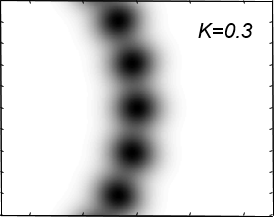
\includegraphics[width=\linewidth]{blanco2008efficient_fig17a}
		\caption{}
		\label{fig:blanco2008efficient_fig17a}
	\end{subfigure}
	\hfill
	\begin{subfigure}[t]{0.24\linewidth}
		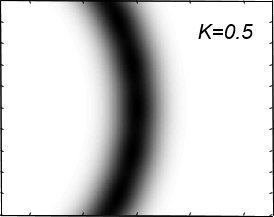
\includegraphics[width=\linewidth]{blanco2008efficient_fig17b}
		\caption{}
		\label{fig:blanco2008efficient_fig17b}
	\end{subfigure}
	\hfill
	\begin{subfigure}[t]{0.24\linewidth}
		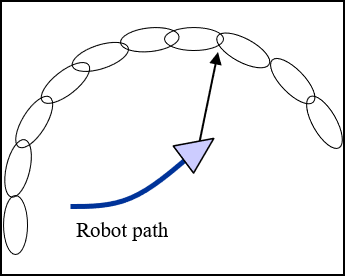
\includegraphics[width=\linewidth]{blanco2008efficient_fig10a}
		\caption{}
		\label{fig:blanco2008efficient_fig10a}
	\end{subfigure}
	\hfill
	\begin{subfigure}[t]{0.24\linewidth}
		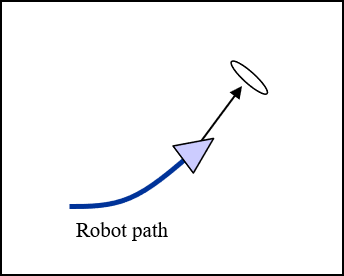
\includegraphics[width=\linewidth]{blanco2008efficient_fig10b}
		\caption{}
		\label{fig:blanco2008efficient_fig10b}
	\end{subfigure}
	\caption{Modellierung der ringförmigen Verteilung über radial angeordnete Normalverteilungen.}
	\label{fig:blanco2008efficient}
	\source{\cite{blanco2008efficientppt}}
\end{figure}


\begin{comment}
--------------------------------------------------------------------------------
- \cite{djugash2009robust}
	- A robust method of localization and mapping using only range
\end{comment}
\section{A robust method of localization and mapping using only range}

Jede bisherige Veröffentlichung die einen \Gls{roslam} mittels eines \Gls{ekf} umsetzen will, muss mit dem Problem der Linearisierung und der Multimodalität der Verteilung kämpfen. Hierfür wurde das Problem bisher immer im kartesischen Koordinatensystem betrachtet. Die Autoren dieses Werkes \cite{djugash2009robust} sind einen anderen Weg gegangen und haben das Problem ins Polarkoordinatensystem überführt. Dieses Vorgehen hat den großen Vorteil, dass ringförmige Verteilungen sehr gut im Polarkoordinatensystem modelliert werden können. Auch ist eine Vorverarbeitung (engl. Batch Process) der Entfernungsmessungen nicht mehr notwendig. Die Ergebnisse der Messung kann direkt an den Filter übergeben werden.

Wie bereits im Grundlagenkapitel besprochen besteht der Zustandsvektor eines \Gls{ekf} für die Lokalisierung aus der Pose (Position und Orientierung) des Roboters:

\[ q_k = \left[ x_k^r, y_k^r, \phi_k^r \right]^T. \]

Für das \Gls{slam} Problem muss der Zustandsvektor um die Positionen der Tags erweitert werden:

\[ q_k = \left[ x_k^r, y_k^r, \phi_k^r, x_k^1, y_k^1, \dots, x_k^N, y_k^N \right]^T. \]

Die Beschreibung des Zustandsvektors in Polarkoordinaten erfolgt dabei über die Festlegung der Mitte des Polarkoordinatensytems $\left( c_{x,k}, c_{y,k} \right)$ und über die Entfernung und den Winkel $\left( r_k, \theta_k \right)$:

\[ q_k = \left[ c_{x,k}^r, c_{y,k}^r, r_k^r, \theta_k^r, \phi_k^r, c_{x,k}^1, c_{y,k}^1, r_k^1, \theta_k^1, \dots, c_{x,k}^N, c_{y,k}^N, r_k^N, \theta_k^N \right]^T .~\footnote{Da für die Beschreibung der Zustände deutlich mehr Parameter benötigt werden, bezeichnet man dieses auch als relative Überparameterisierung (engl. \acrfull{rop}).}\]

Damit können alle Tags beschrieben werden, für den Roboter benötigt man aber noch den zusätzlichen Parameter $\phi_k^r$ um die Ausrichtung (engl. Heading) festzulegen.

Das vorherige Bewegungsmodell (engl. Motion Model) für das kartesischen Koordinatensystem kann weiterverwendet werden, nur die Parameterzuweisungen an $\left( c_{x,k}^r, c_{y,k}^r, \phi_k^r \right)$ ändern sich. Einzig das Messmodell (engl. Measurement Model) muss angepasst werden, um die erwartete Entfernung zu berechnen. Hierfür findet eine Konvertierung der Polarkoordinaten in Kartesische Koordinaten statt.

Die Abbildungen~\ref{fig:djugash2009robust_fig1} verdeutlichen zum einen, wie die Verteilung in Polarkoordinaten dargestellt wird und zum andern, wie mehrere Messungen miteinander kombiniert werden.

\autoref{fig:djugash2009robust_fig1a} beschreibt die tatsächliche Verteilung einer Einzelmessung. Das blaue Rechteck repräsentiert die Roboterposition und der rote Diamant die tatsächliche Tagposition. Die tatsächliche Verteilung einer Einzelmessung wird in Polarkoordinaten als grüne Fläche modelliert, siehe \autoref{fig:djugash2009robust_fig1b}. Über die blaue Ellipse wird die tatsächliche Verteilung mittels einer Normalverteilung angenähert und ergibt dabei die ringförmige Verteilung in der \autoref{fig:djugash2009robust_fig1c}.

Nachdem zwei Messungen von verschiedenen Positionen aus durchgeführt wurden, ergibt sich die tatsächliche Verteilung aus den beiden Schnittpunkten der Ringe, siehe \autoref{fig:djugash2009robust_fig1d}. Die Multimodalität der Verteilung kann über einen \Gls{ekf} nicht mehr abgebildet werden, daher wird zu diesem Zeitpunkt pro Verteilung ein eigener \Gls{ekf} angelegt. \autoref{fig:djugash2009robust_fig1e} beschreibt wie im vorherigen Abschnitt die tatsächlichen und angenäherten Verteilungen in Polarkoordinaten und \autoref{fig:djugash2009robust_fig1f} die Verteilung die sich aus der Annäherung der Verteilung ergibt.

\begin{figure}[h]
	\centering
	\begin{subfigure}[b]{0.32\textwidth}
		\centering
		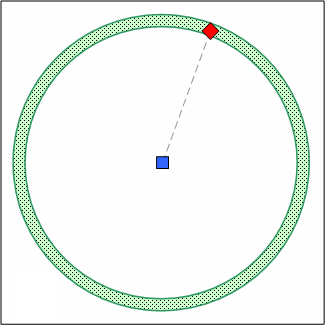
\includegraphics[width=\textwidth]{djugash2009robust_fig1a}
		\caption{}
		\label{fig:djugash2009robust_fig1a}
	\end{subfigure}
	\hfill
	\begin{subfigure}[b]{0.26\textwidth}
		\centering
		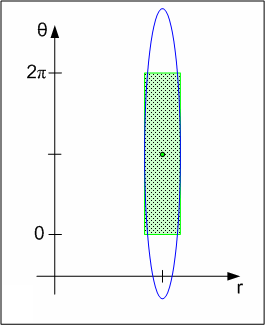
\includegraphics[width=\textwidth]{djugash2009robust_fig1b}
		\caption{}
		\label{fig:djugash2009robust_fig1b}
	\end{subfigure}
	\hfill
	\begin{subfigure}[b]{0.32\textwidth}
		\centering
		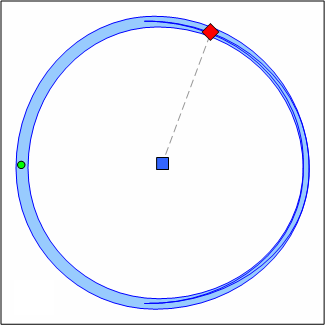
\includegraphics[width=\textwidth]{djugash2009robust_fig1c}
		\caption{}
		\label{fig:djugash2009robust_fig1c}
	\end{subfigure}
	\bigskip
		\begin{subfigure}[b]{0.32\textwidth}
		\centering
		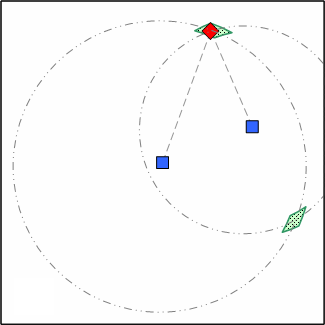
\includegraphics[width=\textwidth]{djugash2009robust_fig1d}
		\caption{}
		\label{fig:djugash2009robust_fig1d}
	\end{subfigure}
	\hfill
	\begin{subfigure}[b]{0.26\textwidth}
		\centering
		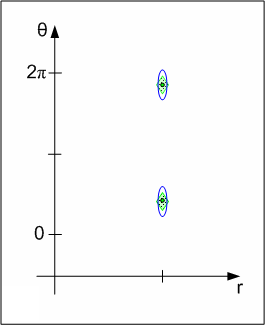
\includegraphics[width=\textwidth]{djugash2009robust_fig1e}
		\caption{}
		\label{fig:djugash2009robust_fig1e}
	\end{subfigure}
	\hfill
	\begin{subfigure}[b]{0.32\textwidth}
		\centering
		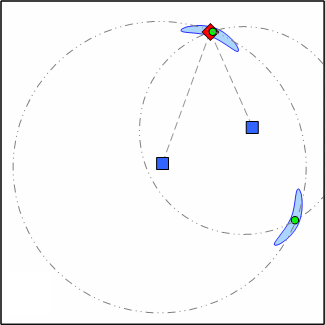
\includegraphics[width=\textwidth]{djugash2009robust_fig1f}
		\caption{}
		\label{fig:djugash2009robust_fig1f}
	\end{subfigure}
	\caption{Darstellung der tatsächlichen und angenäherten Verteilung in Kartesischen und Polarkoordinaten.}
	\label{fig:djugash2009robust_fig1}
	\source{\cite{djugash2009robust}}
\end{figure}


\begin{comment}
--------------------------------------------------------------------------------
- \cite{ahmad2011newstatevector}
	- A New State Vector for Range-Only SLAM
\end{comment}
\section{A New State Vector for Range-Only SLAM}


\begin{comment}
--------------------------------------------------------------------------------
- \cite{herranz2014comparison}
	- A Comparison of SLAM Algorithms with Range Only Sensors
\end{comment}
\section{A Comparison of SLAM Algorithms with Range Only Sensors}




\begin{comment}
------------------------------------------------------------------------------------------
\section{Übersicht der Meilensteine [Remove in final version]}

\begin{description}

\item[2001]
\begin{itemize}
\item !A solution to the simultaneous localization and map building (SLAM) problem (Zitiert von: 2803)
\item +Auxiliary variable based particle filters (115)
\item +Factor graphs and the sum-product algorithm (5869)
\item +Rao-Blackwellised particle filtering for dynamic Bayesian networks (1264)
\end{itemize}

\item[2002]
\begin{itemize}
\item +FastSLAM: A factored solution to the simultaneous localization and mapping problem (2469)
\item Indoor geolocation science and technology (985)
\end{itemize}

\item[2003]
\begin{itemize}
\item !Experimental results in range-only localization with radio (82)
\item !Pure range-only sub-sea SLAM (174)
\item +Recent results in extensions to simultaneous localization and mapping (18)
\end{itemize}

\item[2004]
\begin{itemize}
\item !Tracking moving devices with the cricket location system (547)
\item !A probabilistic approach to inference with limited information in sensor networks (42)
\item +An introduction to factor graphs (672)
\end{itemize}

\item[2006]
\begin{itemize}
\item !Simultaneous localization and mapping: part I (2982)
\item !Simultaneous localization and mapping (SLAM): Part II (1479)
\item Further results with localization and mapping using range from radio (69)
\item !Range-only slam for robots operating cooperatively with sensor networks (146)
\item !Range-only slam with interpolated range data (28)
\end{itemize}

\item[2007]
\begin{itemize}
\item !Application of UWB and GPS technologies for vehicle localization in combined indoor-outdoor environments (52)
\item +Rao-Blackwellized particle filter for multiple target tracking (264)
\end{itemize}

\item[2009]
\begin{itemize}
\item !Navigating with ranging radios: Five data sets with ground truth (18)
\item !Mobile robot localization based on ultra-wide-band ranging: A particle filter approach (90)
\item !Range-only SLAM with a mobile robot and a wireless sensor networks (109)
\end{itemize}

\item[2010]
\begin{itemize}
\item !Geolocation with range: Robustness, efficiency and scalability (11)
\item !Studying of WiFi range-only sensor and its application to localization and mapping systems (3)
\item !tinySLAM: A SLAM algorithm in less than 200 lines C-language program (62)
\end{itemize}

\item[2011]
\begin{itemize}
\item Ultra wide-band localization and SLAM: A comparative study for mobile robot navigation (17)
\item !A new state vector for range-only SLAM (10)
\end{itemize}

\item[2013]
\begin{itemize}
\item A Spectral Learning Approach to Range-Only {SLAM} (13)
\end{itemize}

\item[2014]
\begin{itemize}
\item !A comparison of slam algorithms with range only sensors (2)
\item !Efficient robot-sensor network distributed seif range-only slam (16)
\end{itemize}

\item[2015]
\begin{itemize}
\item ?Fusing ultra-wideband range measurements with accelerometers and rate gyroscopes for quadrocopter state estimation (30)
\end{itemize}

%\item[]
%\begin{itemize}
%\item 
%\end{itemize}

\end{description}
\end{comment}